%----------------------------------------------------------------------------------------
%	PACKAGES AND THEMES
%----------------------------------------------------------------------------------------
\PassOptionsToPackage{table}{xcolor}
\documentclass[aspectratio=169,xcolor=dvipsnames,svgnames,x11names,fleqn]{beamer}
% \documentclass[aspectratio=169,xcolor=dvipsnames,fleqn]{beamer}

\usetheme{RedVelvet}

\usefonttheme[onlymath]{serif}



\usepackage{xspace}
\usepackage{amsmath}
\usepackage{amssymb}
\usepackage{amsfonts}
\usepackage{color}
\usepackage{physics}
% \usepackage{mathbb}
\usepackage{rahul_math}
\usepackage{bigints}
\usepackage{hyperref}

\usepackage{graphicx} % Allows including images
\usepackage{booktabs} % Allows the use of \toprule, \midrule and \bottomrule in tables
\usepackage{tikz,pgfplots}
\usepackage{subfigure}
\usetikzlibrary{arrows}
\usepackage{minted}
\definecolor{LightGray}{gray}{0.9}
\definecolor{cream}{rgb}{0.92, 0.9, 0.55}
\definecolor{lightblue}{rgb}{0.68, 0.85, 0.9}


\usepackage{xcolor-material}
\usetikzlibrary{fit}
\tikzset{%
apple/.pic={
  \fill [MaterialBrown] (-1/8,0)  arc (180:120:1 and 3/2) coordinate [pos=3/5] (@)-- ++(1/6,-1/7)  arc (120:180:5/4 and 3/2) -- cycle;
  \fill [MaterialLightGreen500] (0,-9/10)  .. controls ++(180:1/8) and ++(  0:1/4) .. (-1/3,  -1) .. controls ++(180:1/3) and ++(270:1/2) .. (  -1,   0) .. controls ++( 90:1/3) and ++(180:1/3) .. (-1/2, 3/4) .. controls ++(  0:1/8) and ++(135:1/8) .. (   0, 4/7)
}
}

\newcommand{\leftdoublequote}{\textcolor{blue}{\scalebox{3}{``}}}

\newcommand{\rightdoublequote}{\textcolor{blue}{\scalebox{3}{''}}}


\usepackage{textcomp}
\usepackage{fontawesome}

\usepackage{overpic}

%----------------------------------------------------------------------------------------
%	TITLE PAGE
%----------------------------------------------------------------------------------------

\usepackage{tikz-qtree,tikz-qtree-compat}
\usetikzlibrary{calc}


\title[CPE 381: Signals and Systems]{CPE 381: Fundamentals of Signals and Systems for Computer Engineers} % The short title appears at the bottom of every slide, the full title is only on the title page
\subtitle{07 Sampling Theorem}

\author[Rahul Bhadani] {{\Large \textbf{Rahul Bhadani}}}

\institute[UAH] % Your institution as it will appear on the bottom of every slide, maybe shorthand to save space
{
    Electrical \& Computer Engineering,  The University of Alabama in Huntsville
}
\date

% \titlegraphic{
%    \includegraphics[width=0.4\linewidth]{figures/UAH_primary.png}
% }

\begin{document}

%-------------------------------------------------
\begin{frame}
\titlepage
\end{frame}

%-------------------------------------------------
\begin{frame}{Outline}
    \tableofcontents
\end{frame}


%%%%%%%%%%%%%%%%%%%%%%%%%%%%%%%%%%%%%%%%%%%%%%%%%%%%%
\section{Motivation}

%-----------------------------------------

\begin{frame}{}
    \begin{center}
    \Huge \bf \color{DarkBlue}
    \faFire
    
    Motivation
\end{center}
\end{frame}


\begin{frame}{Motivation}
    \begin{itemize}
        \item Nature has continuous signals.
        \item In order to process them using computers, we need them to sample, quantize, and code to obtain digital signals – both in time and amplitude.
    \end{itemize}
\end{frame}

\begin{frame}{Uniform Sampling}
    Discretize the time-variable
    $$
    x(nT_s) = x(t)\bigg|_{t = nT_s}
    $$
    where $n$ is an integer.
    \begin{center}
             \includegraphics[width=0.50\linewidth, trim={0cm 0.0cm 0cm 0.0cm},clip]{figures/Discretize_Siganl.pdf}
    \end{center}

    \textbf{Sampling processing can be thought of as a modulation processing coming from Pulse Amplitude Modulation, with $\Delta << T_s$; $\Delta$: width of the pulse, $T_s$: sampling period.}
\end{frame}

\begin{frame}{Pulse Amplitude Modulation (PAM)}

\begin{columns}
\column{0.2\linewidth}
    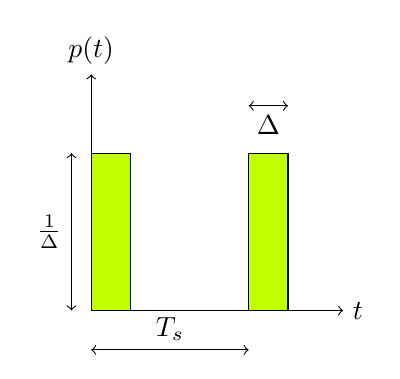
\begin{tikzpicture}
  % Define the pulse width, height, and period
  \def\Deltaval{0.5}
  \def\pulseheight{1/\Deltaval}
  \def\period{2}

  % Draw the x-axis
  \draw[->] (0,0) -- (3.2,0) node[right] {$t$};

  % Draw the y-axis
  \draw[->] (0,0) -- (0,3) node[above] {$p(t)$};

  % Draw the pulse train
  \foreach \i in {0,2} {
    \draw[fill=lime] (\i,0) rectangle (\i+\Deltaval,\pulseheight);
  }

  % % Add x-axis ticks
  % \foreach \i in {0,2,4,6} {
  %   \draw (\i,0) -- (\i,-0.1) node[below] {$\i$};
  % }

  % Draw arrow for sampling time
  \draw[<->] (0,-0.5) -- (2,-0.5) node[midway,above] {$T_s$};

  % Add label for pulse height
  \draw[<->]  (-0.25,0) -- (-0.25,\pulseheight) node[midway,left] {$\frac{1}{\Delta}$};

  % Add label for pulse width
  \draw[<->]  (2,0.6+\pulseheight) -- (2+\Deltaval,0.6+\pulseheight) node[midway,below] {$\Delta$};
\end{tikzpicture}

\column{0.1\linewidth}
{
~~~~~\Huge
\faRemove
}

\column{0.2\linewidth}
\includegraphics[width=1.0\linewidth, trim={0cm 0.0cm 0cm 0.0cm},clip]{figures/Sine.pdf}


\column{0.2\linewidth}
{
\huge
\faArrowRight ~~ \color{black}PAM
}


\end{columns}
\vspace{10pt}
PAM can be thought of as a switch that closes every $T_s$ seconds $\Delta$ seconds and remains open otherwise. PAM $x_{\textrm{PAM}}$ is a multiplication of a continuous-time signal $x(t)$ by a periodic pulse $p(t)$.
\end{frame}

\begin{frame}{PAM}
\small
    For a small pulse width $\Delta$, PAM signal is
    $$
    x_{\textrm{PAM}}(t) = x(t)p(t) = \cfrac{1}{\Delta}\sum_{m}x(mT_s)[u(t-mT_s) - u(t-mT_s - \Delta)]
    $$
As periodic signal can be written as a Fourier series:
$$
p(t) = \suminf{k}P_k e^{jk\Omega_0 t}, \quad \Omega_0 = \cfrac{2\pi}{T_s}
$$
where $P_k$ are the Fourier series coefficients. Hence, the PAM signal can be written as:
$$
x_{\textrm{PAM}}(t) = \suminf{k}P_k x(t)e^{jk\Omega_0 t}
$$
Its Fourier transform is
$X_{\textrm{PAM}}(\Omega) = \suminf{k}P_k X(\Omega - k \Omega_0)$ (using frequency-shift property).

\end{frame}

%%%%%%%%%%%%%%%%%%%%%%%%%%%%%%%%%%%%%%%%%%%%%%%%%%%%%
\section{Sampling Theorem}

%-----------------------------------------

\begin{frame}{}
    \begin{center}
    \Huge \bf \color{DarkBlue}
    \faBraille
    
    Sampling Theorem
\end{center}
\end{frame}


\begin{frame}{Modeling Sampled Signal using Impulses}
    If $\Delta \to 0$, we have a train of impulses. In the limiting conditions, we define the impulse \textbf{sampling function} as

    $$
    \delta_{T_s}(t) = \sum_n\delta(t - nT_s)
    $$
    Thus, the sampled signal is:

    $$
    x_s(t) = x(t)\delta_{T_s}(t)
    $$
\end{frame}


\begin{frame}{}

    \begin{columns}
\column{0.2\linewidth}
    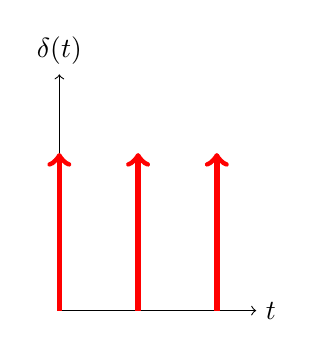
\begin{tikzpicture}
  % Define the pulse width, height, and period
  \def\Deltaval{0.5}
  \def\pulseheight{1/\Deltaval}
  \def\period{1}

  % Draw the x-axis
  \draw[->] (0,0) -- (2.5,0) node[right] {$t$};

  % Draw the y-axis
  \draw[->] (0,0) -- (0,3) node[above] {$\delta(t)$};

  % Draw the pulse train
  \foreach \i in {0,1,2} {
   \draw[thick, ->, red, line width=2pt] (\i,0) -- (\i,\pulseheight);
  }


\end{tikzpicture}

\column{0.1\linewidth}
{
~~~~~\Huge
\faRemove
}

\column{0.2\linewidth}
\includegraphics[width=1.0\linewidth, trim={0cm 0.0cm 0cm 0.0cm},clip]{figures/Sine.pdf}

\column{0.1\linewidth}
{
~~~~~\Huge
\faArrowRight 
}

\column{0.2\linewidth}
{
\includegraphics[width=1.0\linewidth, trim={0cm 0.0cm 0cm 0.0cm},clip]{figures/Discretize_Sine.pdf}

}
\end{columns}
\end{frame}


\begin{frame}{Fourier Series of Impulse Train}
    $$\delta_{T_s}(t) = \suminf_{k} D_k e^{jk\Omega_s T}$$
    where $\Omega_s = \cfrac{2\pi}{T_s}$ is the sampling frequency.

    and,

    $$
    D_k = \cfrac{1}{T_s}\int_{-T_s/2}^{T_s/2} \delta_{T_s}(t) e^{-jk\Omega_s t} dt = \cfrac{1}{T_s}\int_{-T_s/2}^{T_s/2} \delta(t) e^{-jk\Omega_s t} dt = \cfrac{1}{T_s}\int_{-T_s/2}^{T_s/2} \delta(t) e^{-j 0 } dt = \cfrac{1}{T_s}
    $$
\end{frame}

\begin{frame}{Sampled Signal in Continuous-Time and Discrete-Time}
Two ways to imagine the sampled signal $x_s(t)$:

\vspace{10pt}

\begin{columns}
    \column{0.5\linewidth}
    \textbf{Continuous-Time Version}
$$x_s(t) = x(t) \delta_{T_s}(t)  = \cfrac{1}{T_s}\suminf{k} x(t) e^{jk\Omega_s t}$$

$$
X_s(\Omega) = \cfrac{1}{T_s}\suminf{k} X(\Omega - k\Omega_s)
$$

\column{0.5\linewidth}
\textbf{Discrete-time Version}
$$
x_s(t) = \suminf{n} x(nT_s) \delta(t-nT_s)
$$

$$
X_s(\Omega) = \suminf{n} x(nT_s) e^{-j\Omega T_s n}
$$
\end{columns}
\end{frame}

\begin{frame}[allowframebreaks]{Nyquist Sampling Rate Condition}
Depending on the maximum frequency present in the spectrum of $x(t)$ and on the chosen sampling frequency $\Omega_s$ (or the sampling period $T_s$) it is possible to have overlaps when the spectrum of $x(t)$ is
shifted and added to obtain the spectrum of the sampled signal $x_s(t)$. 

\begin{columns}
    \column{0.5\linewidth}
    \includegraphics[width=1.0\linewidth, trim={0cm 0.0cm 0cm 0.0cm},clip]{figures/bandlimited_signal.png}

    Band-limited
    
    \column{0.5\linewidth}
    Band-limited signal $x(t)$ with a low-pass spectrum, finite support, i.e. $X(\Omega) = 0$ for $\Omega > \Omega_{\textrm{max}}$.
\end{columns}

\newpage

\footnotesize
\begin{columns}
    \column{0.5\linewidth}
    \includegraphics[width=1.0\linewidth, trim={0cm 0.0cm 0cm 0.0cm},clip]{figures/bandlimited_signal_no_aliasing.png}

    
    \column{0.5\linewidth}
    Sampling frequency $\Omega_s$ such that the spectrum of the sampled signal consists of shifted non-overlapping versions of $\cfrac{1}{T_s}X(\Omega)$. This is only possible when $\Omega_s - \Omega_{\textrm{max}} \geq \Omega_{\textrm{max}} $ or $\Omega_s \geq 2\Omega_{\textrm{max}} $ which is called \boxed{\textbf{Nyquist sampling rate condition}}.

    \vspace{10pt}
    \color{red}
    If $\Omega_s < 2\Omega_{\textrm{max}} $, then when creating
$X_s(\Omega)$ the shifted spectra of $x(t)$ overlap. . In this case, due to the overlap, it will not be possible to recover the original continuous-time signal from the sampled signal, and thus the sampled signal does not share the same information with the original continuous-time signal. This overlapping phenomenon is called \colorbox{blue!20}{\textbf{frequency aliasing}}.
\end{columns}

\end{frame}

\begin{frame}{Sampling $x(t)$ with Infinite Support}
\begin{columns}
    \column{0.5\linewidth}
       \begin{itemize}
        \item The signal is not band-limited.
        \item Aliasing will always be present.
        \item See the figure on the right for the concept of an anti-aliasing filter.
    \end{itemize}
\column{0.5\linewidth}
\includegraphics[width=1.0\linewidth, trim={0cm 0.0cm 0cm 0.0cm},clip]{figures/nonbandlimitedsignal.png}
\end{columns}
 
    \begin{center}
        \begin{gradred}{}
            The only way to sample a non-band-limited signal $x(t)$ without aliasing --- at the cost of losing information provided by the high-frequency components of $x(t)$ --- is by obtaining an approximate signal $x_a(t)$ lacking the high-frequency components of $x(t)$ and thus permitting us to determine a maximum frequency for it. This is accomplished by \colorbox{yellow!40}{\textbf{anti-aliasing filtering}}, commonly used in samplers.
        \end{gradred}
    \end{center}
\end{frame}

\begin{frame}{Example 1}
\begin{gradgreen}
  Consider the signal $x(t) = 2 \cos(2\pi t + \pi/4)$, $0-\infty <t < \infty$, determine if it is bandlimited. Use $T_s = 0.4, 0.5$, and $1$ seconds/sample as sampling periods, and for each of these find out whether the Nyquist sampling rate condition is satisfied and if the sampled signal looks like the original signal or not.
\end{gradgreen}
\end{frame}

\begin{frame}{}
\vspace*{-9\baselineskip}
    \color{LightGray}{Blank space for calculation}
\end{frame}
\begin{frame}{}
\vspace*{-9\baselineskip}
    \color{LightGray}{Blank space for calculation}
\end{frame}
\begin{frame}{}
\vspace*{-9\baselineskip}
    \color{LightGray}{Blank space for calculation}
\end{frame}

\begin{frame}{Example 1: Assessing Nyquist Criteria}

\begin{center}
    \includegraphics[width=0.5\linewidth, trim={0cm 0.0cm 0cm 0.0cm},clip]{figures/Nqyuist_Criteria.png}
\end{center}
\end{frame}

\begin{frame}{Example 2}
\begin{gradyellow}
        Consider the following signals: (i) $x_1(t) = u(t + 0.5) - u(t-0.5)$; (ii) $x_2(t) = e^{-t} u(t)$.

    Determine if they are band-limited or not. If not, determine the frequency for which the energy of the non-band-limited signal corresponds to 99\% of its total energy and use this result to approximate its maximum frequency.
    
\end{gradyellow}
\end{frame}

\begin{frame}{}
\vspace*{-9\baselineskip}
    \color{LightGray}{Blank space for calculation}
\end{frame}
\begin{frame}{}
\vspace*{-9\baselineskip}
    \color{LightGray}{Blank space for calculation}
\end{frame}
\begin{frame}{}
\vspace*{-9\baselineskip}
    \color{LightGray}{Blank space for calculation}
\end{frame}


\begin{frame}{Reconstruction of Original Continuous Signal}
    \begin{columns}
        \column{0.4\linewidth}
        If $\Omega_s > 2 \Omega_{\textrm{max}}$,
        The spectrum of the sampled signal $x_s(t)$ displays a superposition of shifted versions of the spectrum $X(\Omega)$ multiplied by $\cfrac{1}{T_s}$ with no overlaps.

        \column{0.6\linewidth}
        In such a case, we can get continuous signals by passing the sampled signal through an ideal low-pass filter with a frequency response

        \begin{multiequation}
            H_{\ell p} & = \begin{cases}
                T_s, \quad -\Omega_s/2 \leq \Omega \leq \Omega_s /2\\
                0, \quad \text{otherwise}
            \end{cases}
        \end{multiequation}

        Hence, the reconstructed signal in the form of a Fourier transform can be written as
        \begin{multiequation}
            X_r(\Omega) = H_{\ell p} X_s(\Omega) = \begin{cases}
                X(\Omega),  -\Omega_s/2 \leq \Omega \leq \Omega_s /2\\
                0, \quad \text{otherwise}
            \end{cases}
        \end{multiequation}
        
    \end{columns}
\end{frame}

\begin{frame}{The Exact Recovery of the Original Signal May Not be Possible}

\begin{itemize}
    \item Because the continuous-time signal is not exactly band-limited.
\item Sampling is not done exactly at the uniform-rate, some variations always occur.
\item The filter required for the exact recovery is an ideal low-pass filter which in practice cannot be realized.
\item For non-bandlimited signals, we can use an anti-aliasing filter which is a low-pass filter that enforces to generate an approximate signal with maximum frequency.
\end{itemize}
    
\end{frame}

\begin{frame}{Choosing Cutoff Frequency}

\begin{itemize}
    \item The selection of the cutoff frequency depends on the application and the prior knowledge.
    \item Speech signal has frequencies ranging from 100 Hz - 5 kHz. When sampling speech signal, a cutoff frequency of 5 kHz may be chosen, and the sampling rate is set to 10,000 samples/s.
    \item Music signals may range from 0 to 22 kHz. Thus, when sampling music signals, the antialiasing filter cutoff frequency is set to 22 kHz, and the sampling rate may be 44,000 samples/s or higher.
\end{itemize}
    
\end{frame}


\begin{frame}{Signal Reconstruction from Sinc Interpolation}
    Ideal low-pass filter has impulse response:

    \begin{multiequation}
        h_{\ell p} = \cfrac{T_s}{2\pi} \int_{-\Omega_s/2}^{\Omega_s/2} e^{j\Omega t}d\Omega = \cfrac{\sin(\pi t/T_s)}{\pi t/T_s}, \quad \Omega_s =\cfrac{2\pi}{T_s}
    \end{multiequation}

Reconstruction is the convolution of sampled signal and the low-pass filter's impulse response.

\begin{multiequation}
    x_r(t) & = [x_s * h_{\ell p}](t) = \intinf x_s(\tau)h_{\ell p}(t-\tau)d\tau \\
    & = \intinf \bigg[ \suminf{n} x(nT_s)\delta(\tau - nT_s) \bigg]h_{\ell p}(t-\tau)d\tau = \sum_{n} x(nT_s) \cfrac{\sin (\pi (t-nT_s)/T_s) }{\pi (t-nT_s)/T_s} \\
    & =  \sum_{n} x(nT_s) \textrm{sinc}\bigg( \pi (t-nT_s)/T_s \bigg)
\end{multiequation}
    
\end{frame}

\begin{frame}{Signal Reconstruction from Sinc Interpolation}
    Let $t = k T_s$,

\begin{multiequation}
    x_r(kT_s) =  \sum_{n} x(nT_s) \cfrac{\sin(\pi (k-n)) }{\pi (k-n)}= x(kT_s),
\end{multiequation}
        since

        \begin{multiequation}
            \cfrac{\sin(\pi (k-n)) }{\pi (k-n)}= x(kT_s) = \begin{cases}
                1, \quad k -n = 0, \textrm{~~or~~} n= k \\
                0, \quad n\neq k
            \end{cases}
        \end{multiequation}
\end{frame}


\begin{frame}{The Nyquist-Shannon Sampling Theorem}

Consider, a low-pass continuous signal $x(t)$ is band-limited. $X(\Omega) = 0 $ for $|\Omega| > \Omega_{\textrm{max}}$.

\begin{itemize}
    \item The information in $x(t)$ is preserved when the sampled signal $x_s(t)$ with samples $x(nT_s) = x(t) |_{t = nT_s}$ is created with the sampling frequency $\Omega_s = 2\pi/{T_s}$ rad/s such that $\Omega\_s \geq 2\Omega_{\textrm{max}}$ or $f_s = 1/T_s \geq \cfrac{\Omega_{\textrm{max}}}{\pi}$. 
    
    This is called \colorbox{green!30}{\textbf{Nyquist sampling rate condition}}.

    \item $x(t)$ can be reconstructed by using passing the $x_s(t)$ through an ideal low-pass filter with the frequency response 
    $H(\Omega) = T_s$ for $-\Omega_s/2 < \Omega < \Omega_s/2$, and $H(\Omega) = 0$ otherwise.

    \item $2\Omega_{\textrm{max}}$ is called Nyquist sampling frequency. 
    \item $\Omega_s/2$ is called the folding frequency.
\end{itemize}
    
\end{frame}

\begin{frame}{Sampling of Modulated Signals}
\begin{gradyellow}

Sampling of band-pass signals is used in simulations of communication systems and in implementing modulation systems in software-defined radio.
\vspace{5pt}
    For modulated signals, the sampling rate depends on the bandwidth of the message or modulating signal, rather than on the maximum frequency of the modulated signal.
\end{gradyellow}

A modulated signal: $x(t) = m(t)\cos(\Omega_c t)$.

$m(t)$: Message

$\cos(\Omega_c t)$: Carrier

$\Omega_c$: Carrier Frequency

$\Omega_{\textrm{max}}$: Maximum frequency present in the message

$\Omega_c >> \Omega_{\textrm{max}}$
\end{frame}

\begin{frame}{Sampling of Modulated Signals}
The sampling of $x(t)$ with a sampling period Ts generates in the frequency domain a superposition of the spectrum of $x(t)$ shifted in frequency by $\Omega_s$ and multiplied by $\cfrac{1}{T_s}$.

\begin{gradred}
   To avoid aliasing in the frequency domain, i.e. no overlapping of the shifted spectrum,
   \large
   \begin{multiequation}
       (\Omega_c + \Omega_{\textrm{max}}) - \Omega_s < (\Omega_c - \Omega_{\textrm{max}}) \Rightarrow \Omega_s > 2\Omega_{\textrm{max}}
 \textrm{~~or~~} T_s < \cfrac{\pi}{\Omega_{\textrm{max}}}
 \end{multiequation}
   
   
\end{gradred}

\textbf{Hence, the sampling period depends on the bandwidth $\Omega_{\textrm{max}}$} of the actual message $m(t)$.
\end{frame}

\begin{frame}{Sample-and-Hold Sampling}
\begin{columns}
    \column{0.4\linewidth}
    
    A sample-and-hold sampling system acquires a sample and holds it long enough for quantization and coding to be done before the next sample is acquired.
    \column{0.6\linewidth}
    \begin{center}
    \includegraphics[width=1.0\linewidth, trim={0cm 0.0cm 0cm 0.0cm},clip]{figures/Sample-and-hold.png}
\end{center}
\end{columns}
\end{frame}

\begin{frame}{Zero-order Hold (ZOH)}
Zero-order hold filter is an LTI system that facilitates sample-and-hold.

\vspace{10pt}

Its impulse response $h(t)$  is a pulse of desired width $\Delta \leq T_s$.

\vspace{10pt}


The output of the sample-and-hold system is a weighted sequence of shifted versions of the impulse response. 

\vspace{10pt}

\begin{center}
    \begin{gradgreen}
    \begin{center}
           Ideal Sampler: $x_s(t) = x(t) \delta_{T_s}(t)$

          ZOH Output: $y_s(t) = (x_s * h)(t)$.
    \end{center}
    \end{gradgreen}
\end{center}


\end{frame}


\begin{frame}{Spectrum of ZOH sampled signal}
\small
    \begin{center}
           \begin{multiequation}
               y_s(t) & = (x_s * h)(t) = \sum_{n} x(nT_s) h(t - nT_s)
           \end{multiequation}
    \end{center}
Frequency response of $h(t)$ is:
    \begin{center}
           \begin{multiequation}
              H(\Omega) & = \cfrac{e^{-\Delta s / 2}}{s} ( e^{\Delta s / 2} - e^{-\Delta s / 2} ) \bigg|_{s = j\Omega} = \cfrac{\sin(\Delta \Omega/2)}{\Omega/2}e^{-j \Delta \Omega  / 2}\\
          \textbf{Thus,~~~}  Y_s(\Omega) & = X_s(\Omega) H (\Omega) = \bigg[ \cfrac{1}{T_s} \sum_{k} X(\Omega - k \Omega_s) \bigg] H(\Omega) \\ & = X_s(\Omega) H (\Omega) = \bigg[ \cfrac{1}{T_s} \sum_{k} X(\Omega - k \Omega_s) \bigg]  \cfrac{\sin(\Delta \Omega/2)}{\Omega/2}e^{-j \Delta \Omega  / 2}
           \end{multiequation}
    \end{center}
\end{frame}





%%%%%%%%%%%%%%%%%%%%%%%%%%%
\section{Quantization
}
\begin{frame}{}
    \begin{center}
    \Huge \bf \color{DarkBlue}
\faAnchor

    Quantization
\end{center}
\end{frame}




\begin{frame}{Quantization and Coding}

    \begin{columns}
        \column{0.5\linewidth}

        \begin{itemize}
            \item Amplitudes are quantized – they have certain levels.
\item To facilitate the quantization, we have a quantizer.
\item A quantizer is a nonlinear system.

\item \color{SeaGreen} Number of quantization levels is specified by how many bits we use to encode.

\item \color{DodgerBlue4} Of course, quantization introduces error as quantization is merely an approximation. The error is called \textbf{quantization error}.
        \end{itemize}

        \column{0.5\linewidth}
       \includegraphics[width=1.0\linewidth, trim={0cm 0.0cm 0cm 0.0cm},clip]{figures/Quantized_Sine.pdf}
       \footnotesize
       \textbf{Code:} \url{https://github.com/rahulbhadani/CPE381_FA26/blob/main/Code/Ch07_quantizing_signal.m}
    \end{columns}
    
\end{frame}

\begin{frame}{Quantization Step}
    \begin{columns}
        \column{0.5\linewidth}
        $$
        \Delta = \cfrac{\textrm{dynamic range of signal}}{2^b}
        $$
        \column{0.5\linewidth}
        \includegraphics[width=1.0\linewidth, trim={0cm 0.0cm 0cm 0.0cm},clip]{figures/Four_Level_Quantizer.png}
    \end{columns}
\end{frame}

\begin{frame}{Quantization Error}
    Sampled Signal: $x(nT_s) = x(t)|_{t = nT_s}$

    \textbf{Example: 4-level quantizer}

$k\Delta \leq x(nT_s) < (k+1)\Delta \Rightarrow \hat{x}(nT_s)) = k\Delta, \quad k = -2, -1, 0, 1$.

\begin{multiequation}
& & & ~~~~~\hat{x}(nT_s)) & ~~~\Rightarrow~~~ & \textrm{Binary Code}\\
    -2\Delta \leq x(nT_s)< -\Delta & ~~~\Rightarrow~~~ & \hat{x}(nT_s)) = -2\Delta ~~~~|  &~~~~~ -2\Delta & 10\\
    -\Delta \leq x(nT_s)< 0 & ~~~\Rightarrow~~~ & \hat{x}(nT_s)) = -
        \Delta ~~~~|  &~~~~~~~ -\Delta & 11\\
    0 \leq x(nT_s)< \Delta & ~~~\Rightarrow~~~ & \hat{x}(nT_s)) = 0 ~~~~|  &~~~~~~~~~ 0\Delta & 00\\
    \Delta \leq x(nT_s)< 2\Delta & ~~~\Rightarrow~~~ & \hat{x}(nT_s)) = \Delta ~~~~|  &~~~~~~~~~~ \Delta & 01\\    
\end{multiequation}
    
\end{frame}

\begin{frame}{Quantization Error}
\begin{center}
    We define quantization error as $\varepsilon (nT_s) = x(nT_s) - \xhat(nT_s)$

\begin{gradred}
\begin{center}
     \begin{multiequation}
            \xhat(nT_s)  \leq x(nT_s) & \leq \xhat(nT_s) + \Delta\\
     0 & \leq \varepsilon(nT_s)\leq \Delta
     \end{multiequation}\
  
\end{center}
   
\end{gradred}
\end{center}    
\end{frame}

\begin{frame}{Example}
    Suppose we are trying to decide between an 8 and a 9-bit A/D converter for a certain application where the signals in this application are known to have frequencies that do not exceed 5 kHz. The dynamic range of the signals is $10 V$, so that the signal is bounded as $-5 \leq x(t) \leq 5$. Determine an appropriate sampling period and compare the percentage of error for the two A/Ds of interest.
    
\end{frame}


\begin{frame}{}
\vspace*{-9\baselineskip}
    \color{LightGray}{Blank space for calculation}
\end{frame}
\begin{frame}{}
\vspace*{-9\baselineskip}
    \color{LightGray}{Blank space for calculation}
\end{frame}
\begin{frame}{}
\vspace*{-9\baselineskip}
    \color{LightGray}{Blank space for calculation}
\end{frame}

\section{Applications}

\begin{frame}{}
    \begin{center}
    \Huge \bf \color{DarkBlue}
    \faWifi
    
    Applications
\end{center}
\end{frame}


\begin{frame}{Application to Digital Communication: PCM}
    \begin{itemize}
        \item Sampling theorem by Nyquist and Shannon led to the era of digital communication.
        \item Modern digital communication using Pulse Code Modulation (PCM).

         \includegraphics[width=0.6\linewidth, trim={0cm 0.0cm 0cm 0.0cm},clip]{figures/Pulse_Code_Modulation.png}
        
    \end{itemize}
\end{frame}



\begin{frame}{Application to Digital Communication: TDM}

   \small
    \begin{itemize}
        \item Pulse-modulated signals have large bandwidths, causing frequency overlap and interference when transmitted together.
        
        \item However, these signals provide information only at the sampling times.
        \item Between these sampling times, samples from other signals can be inserted, generating a combined signal with a smaller sampling time. At the receiver, the samples corresponding to each of the multiplexed signals are separated.
        \item This forms the principle of \colorbox{purple!30}{\textbf{time-division multiplexing (TDM)}}, where pulses from different signals are interspersed into one signal, converted into a PCM signal, and transmitted.
    \end{itemize}
    \begin{center}
           \includegraphics[width=0.6\linewidth, trim={0cm 0.0cm 0cm 0.0cm},clip]{figures/TimeDivisionMultiplexing.png}

    \end{center}
   
\end{frame}


\end{document}